\documentclass[10pt]{article}
\usepackage{float}
\usepackage[utf8]{inputenc}
\usepackage[OT1]{fontenc}
\usepackage{amsfonts, amsmath, amsthm, amssymb}
\usepackage{bbm}
\usepackage{mathtools}
\usepackage{natbib}
\usepackage{graphicx}
\usepackage{listings}
\usepackage[margin=1in]{geometry}
\usepackage{xcolor}
\usepackage{bigints}
\usepackage{glossaries}
\usepackage{graphicx}
\usepackage{enumerate}

\theoremstyle{definition}
\newtheorem{definition}{Definition}[section]

\newtheorem{theorem}{Theorem}
\newtheorem{proposition}{Proposition}
\newtheorem{example}{Example}

\newcounter{countCode}
\lstnewenvironment{code} [1][caption=Ponme caption, label=default]{%
	\renewcommand*{\lstlistingname}{Listado} 
	\setcounter{lstlisting}{\value{countCode}} 
	\lstset{ %
	language=java,
	basicstyle=\ttfamily\footnotesize,       % the size of the fonts that are used for the code
	numbers=left,                   % where to put the line-numbers
	numberstyle=\sc,      % the size of the fonts that are used for the line-numbers
	stepnumber=1,                   % the step between two line-numbers. 
	numbersep=5pt,                 % how far the line-numbers are from the code
	numberstyle=\color{red!50!blue},
    	backgroundcolor=\color{lightgray!20},
	rulecolor=\color{blue},
	keywordstyle=\color{red}\bfseries,
	showspaces=false,               % show spaces adding particular underscores
	showstringspaces=false,         % underline spaces within strings
	showtabs=false,                 % show tabs within strings adding particular underscores
	frame=single,                   % adds a frame around the code
	framexleftmargin=0mm,
	numberblanklines=false,
	xleftmargin=5pt,
	breaklines=true,
	breakatwhitespace=true,
	breakautoindent=true,
	captionpos=t,
	texcl=true,
	tabsize=2,                      % sets default tabsize to 3 spaces
	extendedchars=true,
	inputencoding=utf8, 
	escapechar=\%,
	morekeywords={print, println, size, background, strokeWeight, fill, line, rect, ellipse, triangle, arc, save, PI, HALF_PI, QUARTER_PI, TAU, TWO_PI, width, height,},
	emph=[1]{print,println,}, emphstyle=[1]{\color{blue}}, % Mis palabras clave.
	emph=[2]{width,height,}, emphstyle=[2]{\bf\color{violet}}, % Mis palabras clave.
	emph=[3]{PI, HALF_PI, QUARTER_PI, TAU, TWO_PI}, emphstyle=[3]\color{orange!50!violet}, % Mis palabras clave.
	emph=[4]{line, rect, ellipse, triangle, arc,}, emphstyle=[4]\color{green!70!black}, % Mis palabras clave.
	%emph=[5]{size, background, strokeWeight, fill,}, emphstyle=[5]{\tt \color{red!30!blue}}, % Mis palabras clave.
	%emph={[2]sqrt,baset}, emphstyle={[2]\color{blue}}, % f(sqrt(2)), sqrt a nivel 2 se pondrá azul
	#1}}{\addtocounter{countCode}{1}}



\title{Dataset Transferability Analysis via Optimal Transport}
\author{Davi Sales Barreira}
\date{\today}
\begin{document}
\maketitle

\section{Introduction}

Optimal Transport (OT) theory is a field of mathematics that studies the problem of optimally transporting
quantities from one configuration to another given a cost function.
The origin of the field is commonly attributed to the french mathematicians Gaspard Monge (1746-1818)
whose original motivating problem was
``what is the optimal way to transport soil extracted
from one location and move to another where it will be used,
for example, on a construction?'' (see Figure \ref{fig:mongeproblem}).

\begin{figure}[H]
  \centering
  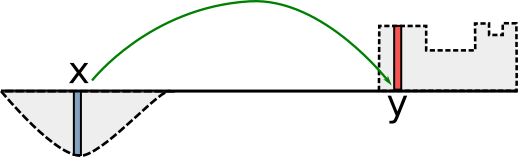
\includegraphics[width=8cm]{Figures/mongeproblem.png}
  \caption{Illustration of the original Monge Problem, where all the mass is excavated from location
  $x$ is transported to a deterministic location $y$.
  The transport assignment map is represented by the arrow in green.}
  \label{fig:mongeproblem}
\end{figure}

This seemingly narrow subject has actually many applications beyond what one may see at first.
In the field of Machine Learning, Optimal Transport theory has been gaining attention, specially
in subareas such as transfer learning
(\citep{flamary2014optimal}, \citep{courty2014domain},
\citep{damodaran2018deepjdot}, \citep{solomon2014wasserstein},
\citep{shen2018wasserstein}).
One of the main ways in which OT is used in Machine Learning is in order to define
a distance metrics between probability distributions. Note that
two datasets may be interpreted as empirical distributions
in high-dimensions, and one can use Optimal Transport in order to obtain the minimal cost
of transporting one dataset distribution into the other. This cost can be thought of
as a distance measure between datasets.

This project is based on the work of \citet{alvarez2020geometric}, where the
authors proposed one way of measuring the distance between datasets using
Optimal Transport. Their metric, which was called Optimal Transport
Dataset Distance (OTDD), was shown to be correlated to performance in terms of
transfer learning, i.e. the lower the OTDD, the better was the transfer learning
between two datasets. Hence, the OTDD could be
used as a parameter to evaluate how well the transfer learning would be
between two datasets.

Suppose that you have many
datasets which you can train to then use a transfer learning method
in order to make prediction in another dataset. Hence,
\citet{alvarez2020geometric} proposed the use of OTDD as a metric
in order to evaluate which dataset would be best suited.

In this project, we make use of the OTDD metric to evaluate
the transferability between two datasets, but instead of
comparing many datasets, we develop a tool that allows users
to explore the differences between the datasets, and perform data
augmentations in order to improve the transferability between the datasets, i.e.
reduce the OTDD distance.

\section{Datasets}

We utilize the MNIST and FashionMNIST (FMNIST) datasets, which are benchmark
datasets for Machine Learning. The MNIST dataset is composed of handwritten
digits from zero to nine, each picture is in gray-scale and consists
in 28 by 28 pixels.
The FMNIST consists of small photos of clothes divided in 10 categories (e.g. shoes, dress, shirt, etc)
Each image is also in gray-scale and 28 by 28 pixels.
Figure \ref{fig:dataset} presents some samples from the datasets.

\begin{figure}[H]
  \centering
  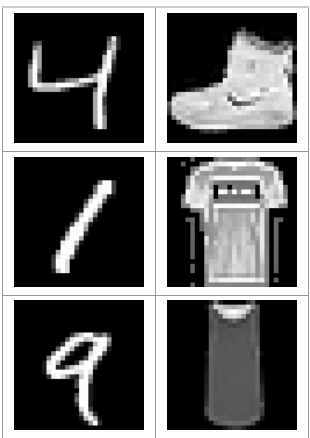
\includegraphics[width=4cm]{Figures/datasets.png}
  \caption{In the left, samples from MNIST. In the right, samples from FMNIST.}
  \label{fig:dataset}
\end{figure}

\section{Technology Used}

This project used the Julia programming language to perform the Optimal Transport
calculations and all the datasets transformations. Also, instead of Observable,
we've utilized a tool called ``Pluto'', which is a notebook in Julia very
similar to Observable. The visualization tool was built inside the Pluto notebook 
which enabled the creations of buttons and interactive calculations.
Similar to Observable, the Pluto notebook does not access directly the data
in the computer, so in order to plot the images from the datasets,
we also shipped a small code in Julia to create a server to serve the data.

Inside Pluto notebook, we wrote javascript code with instruction to create
the visualization graphs with D3 and VegaLite.

\section{Visualization Tool}

The visualization tool developed in this project has three main components.
The first one, shown in Figure \ref{fig:mainscreen}, is composed of two views.
In the view in the left, we use the UMAP dimensionality reduction in order to visualize
the datasets in two dimensions.The edges in blue represent the optimal map
for transporting the empirical distribution of one dataset into another.
Note that the OTDD is related to such edges, since it measures the Optimal Transport
distance between the datasets. In this view, the user can use a brush to do a first
selection of the datasets which he wants to perform the data augmentation by pressing
the ``Select Initial Samples'' button.
Also, note that there is a small selector in the top left, where
the user may change the marker type from ``Image'' to ``Circle'', which
will more clearly show which sample belongs to which dataset.

The view on the right contains a heatmap with the dataset labels in each axis.
This heatmap contains the number of samples that are transported in terms
of their labels. Qualitatively, when two datasets have good transferability,
it is expected that such heatmap matrix will be sparse. The reason for this is that
, in the ideal scenario for transfer learning, all samples with the same label
would all be ``transported'' to samples in the second dataset also all with the same
label (e.g. all 1's in MNIST go to ``dresses'' in the FMNIST).
Therefore, the main reason for this view on the right is to help the user
understand which labels have more space for improvement.

\begin{figure}[H]
  \centering
  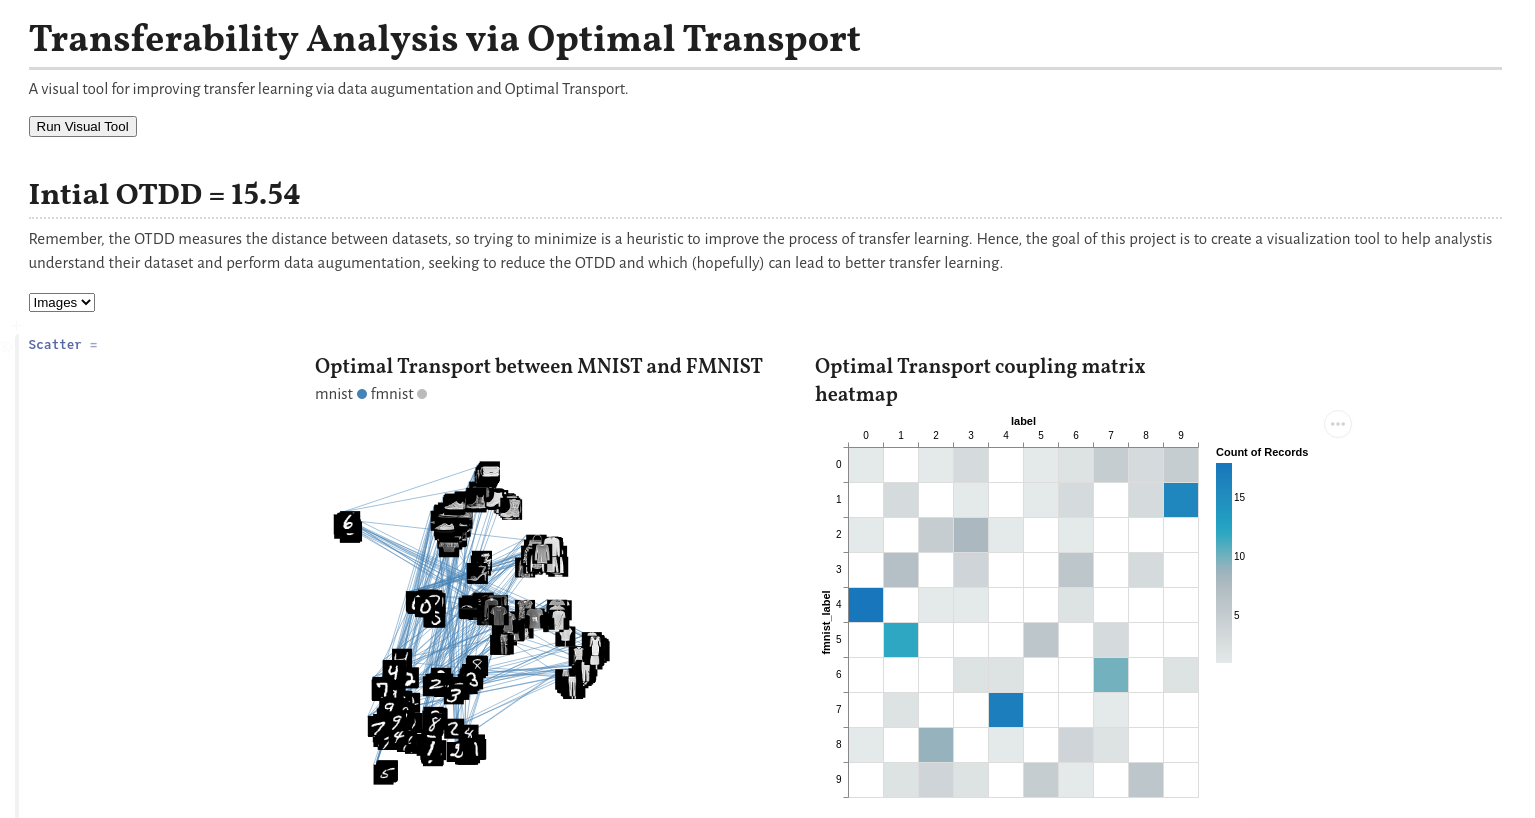
\includegraphics[width=16cm]{Figures/mainscreen.png}
  \caption{In the left, samples from MNIST. In the right, samples from FMNIST.}
  \label{fig:mainscreen}
\end{figure}

The second component is a rescaled view of the data samples selected in the first
component. These samples appear as soon as the user presses the ``Select Initial Sample''
button. In here, the user can do a more thorough visual inspection of the samples.
Here there is also a brush for the user to perform another selection.
Then, by pressing the ``Final Picks'' button, the visual tool selects the samples
inside the brush and sends them to the third component.

\begin{figure}[H]
  \centering
  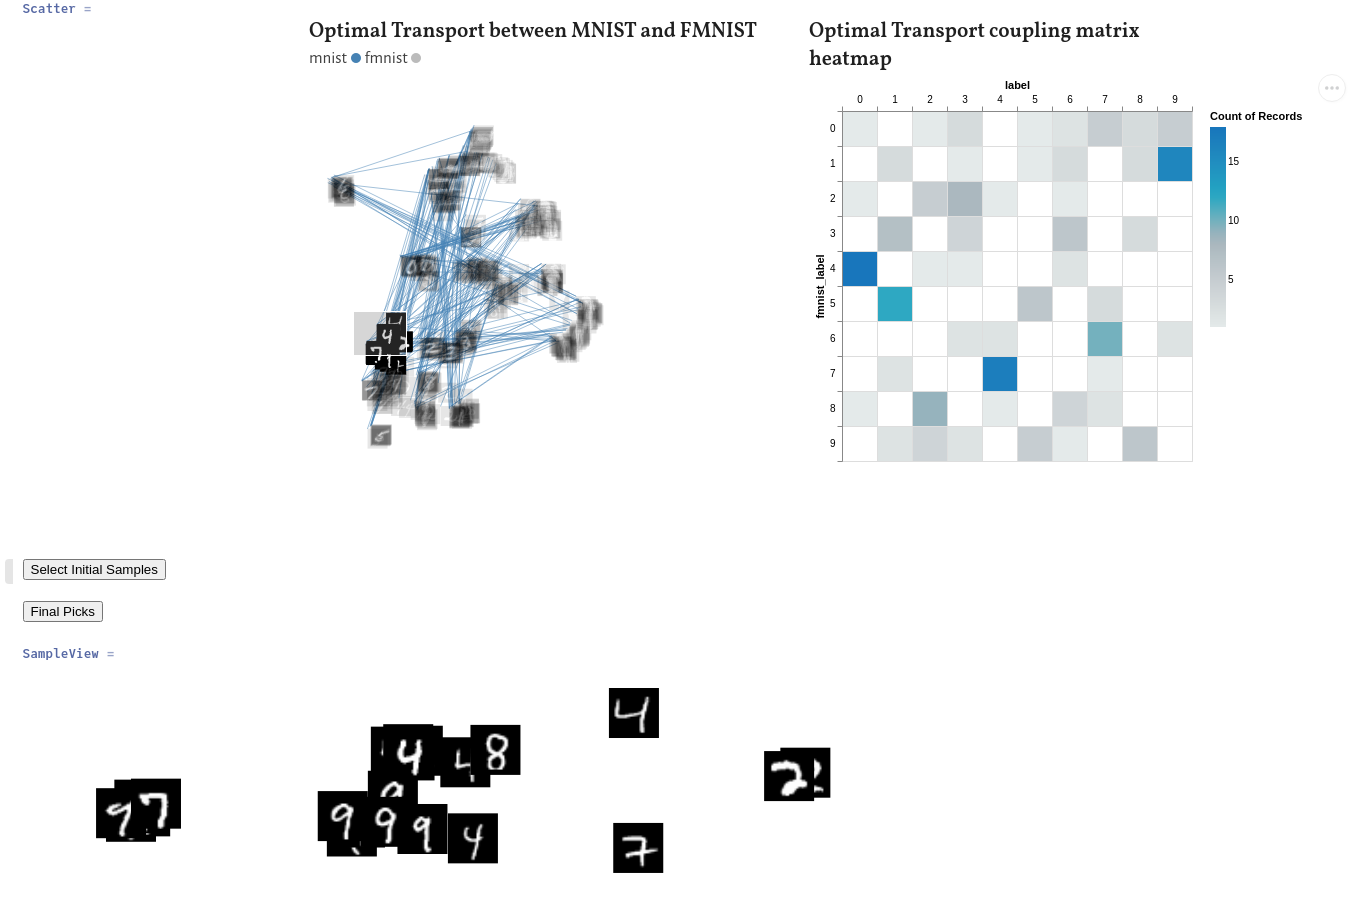
\includegraphics[width=14cm]{Figures/secondscreen.png}
  \caption{Example of user selecting some samples in the first view, and visualizing them
  after pressing the ``Sample Initial Samples'' buttons.}
  \label{fig:secondscreen}
\end{figure}

The third component is where the user will apply the modifications to the samples,
trying to reduce the OTDD and thus, improving the transferability between the datasets.
This component has a ``Default'' button, two sliders and two checkboxes. The first slider performs
an equalization of the data (i.e. it makes images thinner or thicker depending on
the value of gamma applied). The second slider performs rotations.
The checkers perform either vertical or horizontal mirroring. Finally, the ``Default''
button restores the original images.

As the user applies this transformations to the data, there is a view
in the bottom showing how the final samples will look. The OTDD recalculated
as the values in the handles are modified, so the user can visualize in real
time how the modifications are affecting the transferability.

\begin{figure}[H]
  \centering
  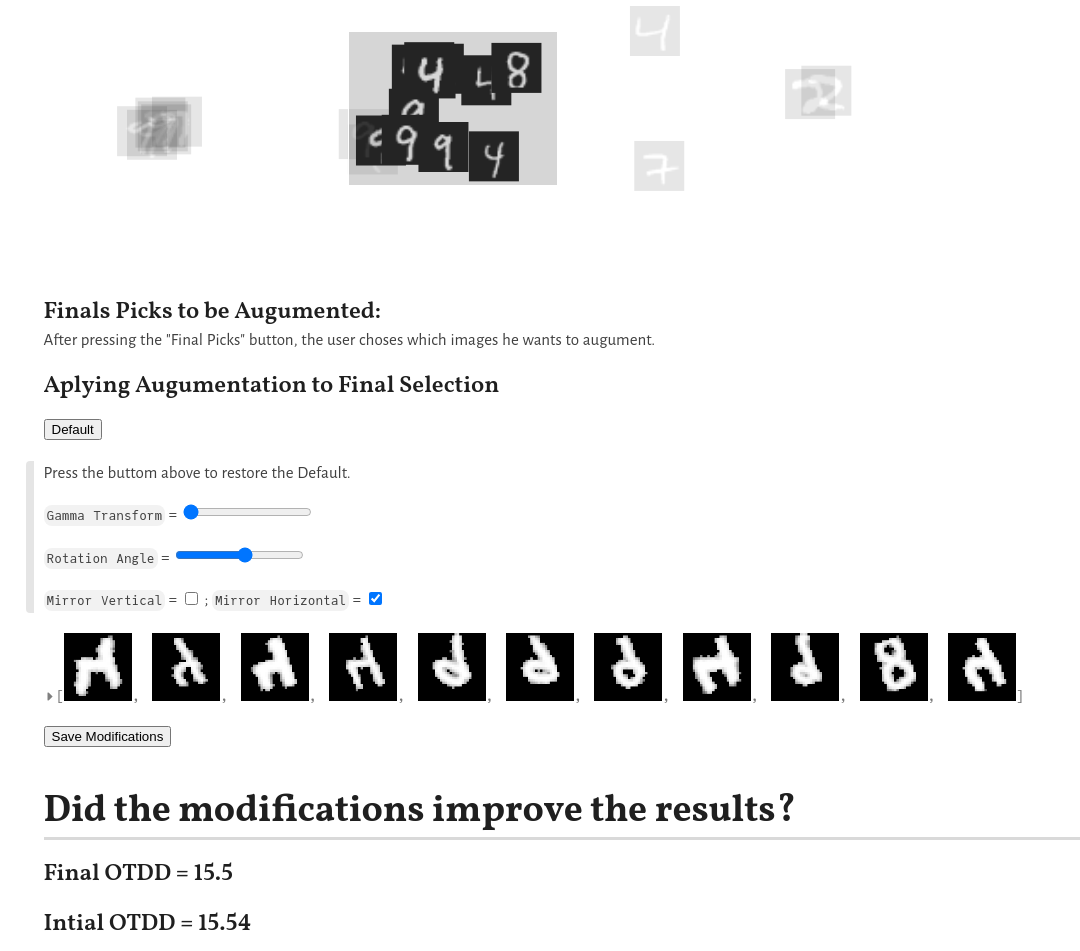
\includegraphics[width=14cm]{Figures/thirdscreen.png}
  \caption{Third component of the visualization tool.}
  \label{fig:thirdscreen}
\end{figure}

\section{Installation and Troubleshooting}

In this section, we give the instructions on how to run the visualization tool
developed in this project, and how to solve possible issues when trying to
run it for the first time.

As we've stated, this project was developed in the Julia programming language,
hence, the user must have Julia installed.

The visualizations use a ``cdn'' to import the javascript packages (i.e. d3 and VegaLite),
therefore, it requires internet access to properly work.

% \nocite{*}

  \bibliography{ref}
  \bibliographystyle{plainnat}
\end{document}

